\documentclass{article}
\usepackage[utf8]{inputenc}

\title{IF672 - Algoritmos e Estrutura de Dados}
\author{Fernando Vilela Brandão }
\date{Outubro, 2019}

\usepackage{natbib}
\usepackage{graphicx}

\begin{document}
\maketitle

\begin{figure}[h!]
\centering
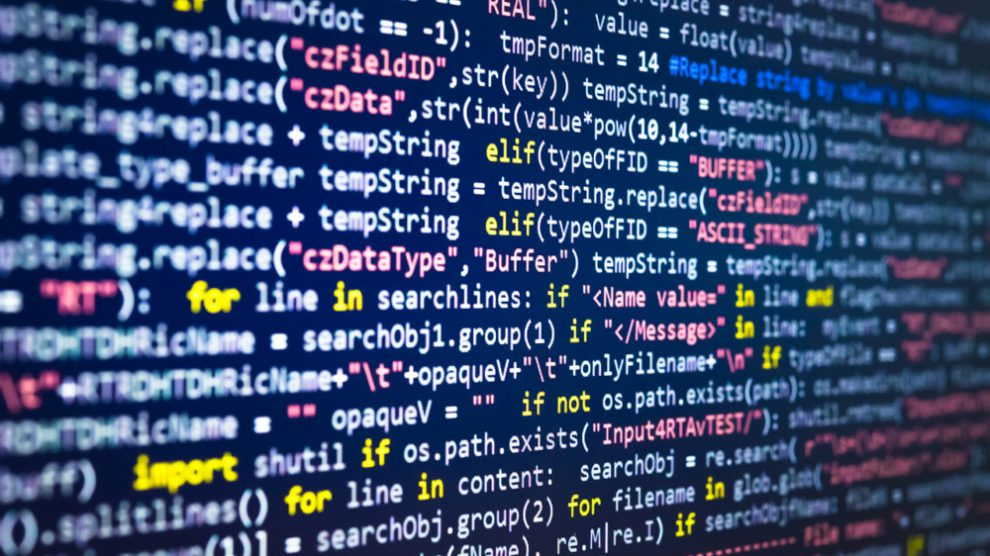
\includegraphics[scale=0.3]{algoritmos-990x556.jpg}
\caption{Exemplo de um algoritmo\citep{algo}}
\label{fig:algoritmos-990x556.jpg}
\end{figure}
\section{Introdução}
Em um mundo cada vez mais informatizado e com sistemas de computadores cada vez mais avançados se torna essencial para qualquer profissional da área da informática ter uma conhecimento profundo de algorítimos. E a cadeira Algoritmos e Estrutura de Dados busca exatamente isso, aprofundar o conhecimento do aluno em seus conhecimentos de programação deixando assim os códigos mais claros e eficientes.
\section{Relevância}
A importância da cadeira Algoritmos e Estrutura de Dados é que no final do semestre se espera que o aluno tenha a capacidade de fazer algorítimos eficientes e claros. De forma que quando estiver inserido no mercado de trabalho  indivíduo tenha capacidade de fazer códigos claros facilitando assim a manutenção dos mesmos.\citep{cinWiki} 
\label{fig:my_label}
\section{Relação com outras disciplinas}

A cadeira Algoritmos e Estrutura de Dados se relaciona diretamente com a cadeira Introdução a Programação do primeiro período. Além do fato da segunda ser um pré requisito da primeira, na Introdução a programação o aluno aprende o que é um algoritmo e como cria-los e na cadeira do segundo período o discente desenvolve esses algoritmos mais eficientes e organizados.\citep{Perfil}
\label{fig:my_label}

\bibliographystyle{plain}
\bibliography{references}
\end{document}

